\documentclass[12pt]{article}
\usepackage[T1]{fontenc}
\usepackage{fancyhdr}
\usepackage{graphicx}
\usepackage{amsmath}
\usepackage{geometry}
\usepackage{caption}
\usepackage{float}
\usepackage{xcolor}
\usepackage{hyperref}
\usepackage{listings}
%\usepackage[listings]{tcolorbox}
\usepackage[most]{tcolorbox}

\lstdefinelanguage{yaml}{
  morekeywords={true,false,null},
  sensitive=false,
  morecomment=[l]{\#},
  morestring=[b]",
  morestring=[b]'
}
\geometry{margin=1in}
\lstset{basicstyle=\ttfamily\small, columns=fullflexible,
  breaklines=true, showstringspaces=false, keepspaces=true,
  aboveskip=3pt, belowskip=3pt}
\tcbset{colback=white, colframe=gray, title=Terminal,
  sharp corners, breakable, top=1mm, bottom=1mm}


%%% TITLE %%%
\title{\textbf{AmigoBot with ROS 1}}
\author{M. J. Khojasteh}
\date{October 2026}
%%% END TITLE %%%

%%% HEADER CONFIGURATION %%%
\setlength{\headheight}{1.5cm}
\addtolength{\topmargin}{-0.5cm}
\pagestyle{fancy}
\fancyhf{}

\fancyhead[L]{\textbf{EEEE-585/685 \\ Lab \#5: AmigoBot}}
\fancyhead[R]{
\includegraphics[height=1cm]{Figures/Formatting/kgcoeLogo.png}}
\fancyfoot[C]{\thepage}
%%% END HEADER CONFIGURATION %%%

\begin{document}

\maketitle
\thispagestyle{fancy}

\section{Objective}
In this experiment, students will use the AmigoBot by MobileRobots to investigate key aspects of mobile robot navigation in ROS 1 Noetic. They will design, simulate, and implement basic navigation algorithms, gaining hands-on experience throughout the process. The experiment also examines the positional errors that arise when using dead reckoning techniques in combination with encoder data.
\vspace{12pt}

\noindent
Upon completion of this lab, students should be able to:
\begin{enumerate}
  \item Use ROS publishers and subscribers to control a differential drive robot and read its sonar and odometry data.
  \item Develop and test motion commands in simulation, then use the same ROS interface on the real robot.
  \item Estimate the robot's pose from wheel velocities and evaluate accumulated dead reckoning error.
\end{enumerate}

\begin{figure}[H]
  \centering
  \begin{minipage}{0.36\textwidth}
    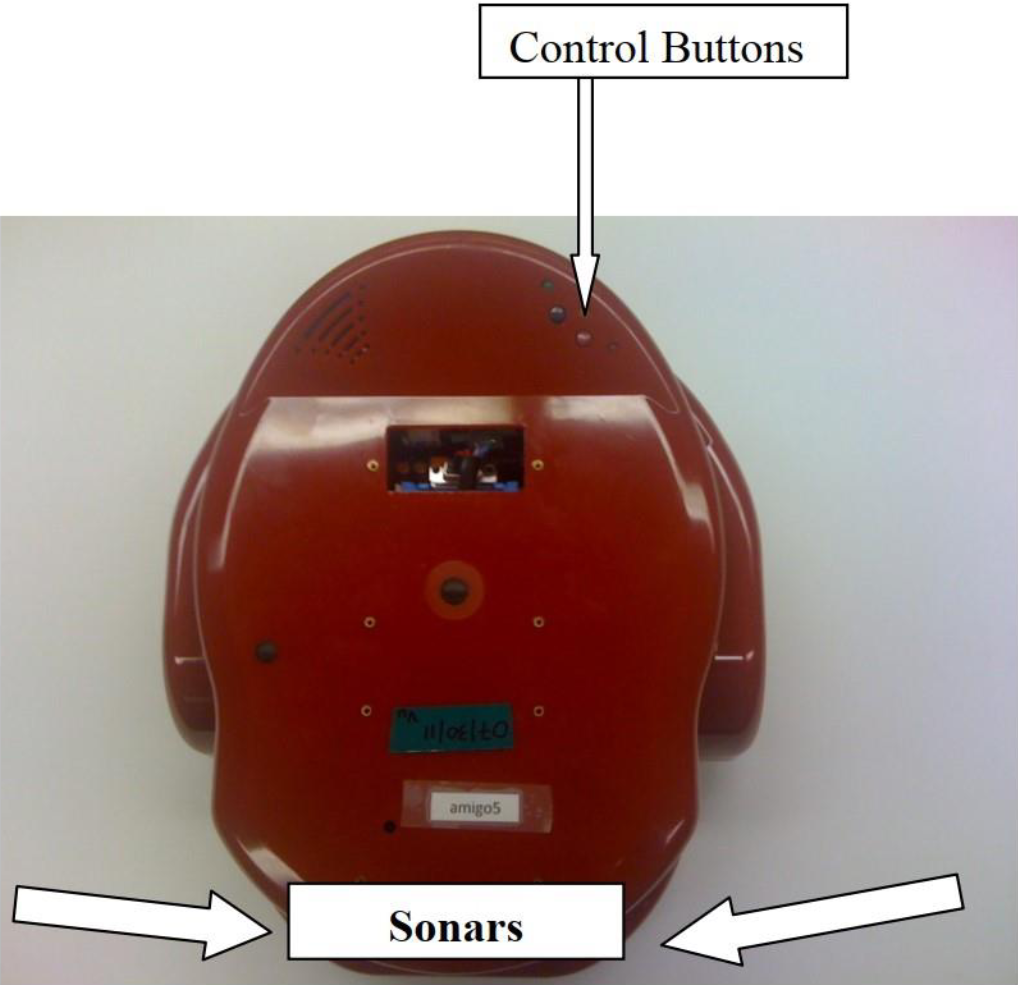
\includegraphics[width=\linewidth]{Figures/Lab5/lab5_amigo.png}
  \end{minipage}\hfill
  \begin{minipage}{0.60\textwidth}
    \small
    \textbf{Technical Specifications}:\\[4pt]
    \textbf{Max forward/backward speed}: 1 m/s;\\
    \textbf{Rotation speed}: $100^\circ$/s;\\
    \textbf{Ultrasonic sensors}: 1 on each side, 4 in front, 2 in the rear;\\
    \textbf{Encoders}: 9,550 ticks per wheel revolution;\\
    \textbf{Microcontroller}: 44 MHz Renesas SH2-7144;\\
    \textbf{Communication ports}: $2\times$ RS-232;\\
    \textbf{Control buttons}: Red (Reset), Black (Motor Test).
  \end{minipage}
\end{figure}

\newpage

\section{Theory}
\subsection*{Dead Reckoning}
Dead reckoning, derived from the term “deduced reckoning” used in navigation, is a method of estimating an object’s current position based on its previous location and known or estimated values of speed, time, or direction of travel. Because positional errors can accumulate over time, dead reckoning is often combined with other navigation techniques to improve accuracy and minimize cumulative error.




\subsection*{Encoders}
Optical encoders, like those used in the AmigoBot, are commonly employed to measure the speed and position of a wheel shaft. They consist of a light source, a fixed grating to modulate the light, a rotating disc with a fine optical pattern attached to the wheel shaft, and stationary optical detectors. As the shaft rotates, the detectors sense varying light levels depending on the alignment of the fixed and rotating gratings.

The AmigoBot provides 9,550 encoder ticks per wheel revolution (approximately 30 ticks per millimetre of travel). Quadrature encoders use two signals offset by 90 degrees to determine shaft movement and direction. In this lab, the provided ROS interface supplies wheel angular velocities in radians per second, so your odometry node does not need to decode raw encoder ticks.




\section{Introduction}
The AmigoBot is a compact, intelligent, two-wheeled differential drive mobile robot and the smallest model in the Pioneer robot family developed by MobileRobots Inc. It is widely used by research institutions around the world for robotics education and experimentation.
\noindent
Designed for autonomous navigation in real-world environments, the AmigoBot is equipped with essential components including a rechargeable battery, drive motors, two main wheels with a supporting caster wheel, position and speed encoders, sonar range sensors, and an onboard microcontroller.


\subsection*{ROS interface with AmigoBot}

\begin{itemize}
  \item The supplied workspace contains five packages: \texttt{amigo\_description} (robot model and parameters), \texttt{amigo\_gazebo} (simulation), \texttt{amigo\_bringup} (real robot), \texttt{amigo\_tools} (interface and test tools), and \texttt{amigo\_student} (task skeletons).
  \item The container includes ROS 1 Noetic, Gazebo 11, ROSARIA and the ARIA robot library. The supplied packages replace the older MABL examples; no additional repository clones or launch-file fixes are needed.
  \item Simulation and hardware provide the same command, sonar, odometry and wheel-velocity topics. Only \texttt{/ground\_truth/state} is exclusive to simulation.
\end{itemize}

\section*{Workspace Setup}

\begin{enumerate}
  \item Install Docker (Docker Desktop on macOS or Windows, or Docker Engine on Linux) and VS Code with the \textbf{Dev Containers} extension.
  \item Open the supplied \texttt{lab5/} folder itself in VS Code. Run \textbf{Dev Containers: Reopen in Container} and wait for the first build to finish. The container builds \texttt{catkin\_ws} automatically.
  \item Open \url{http://localhost:6080} in your browser for the desktop where Gazebo and RViz appear. No separate X server is required.
  \item Run all ROS commands below in VS Code terminals \emph{inside the container}. New terminals start in \texttt{\string~/catkin\_ws} with ROS and the workspace already sourced.
\end{enumerate}

Edit the Python skeletons in \texttt{amigo\_student/scripts/} under
\path{lab5/catkin_ws/src/amigobot_ros/}.
They run but do not implement the tasks until you fill in their TODOs.
Python edits need no rebuild. If you add a Python script, make it executable:

\begin{tcolorbox}
\begin{lstlisting}[language=bash]
chmod +x ~/catkin_ws/src/amigobot_ros/amigo_student/scripts/my_new_node.py
\end{lstlisting}
\end{tcolorbox}

For new packages or compiled-code changes, run \texttt{catkin\_make} in
\texttt{\string~/catkin\_ws}. Then run
\texttt{source devel/setup.bash} in each terminal using it.

\section*{Launching the Simulation}

In one container terminal, run:

\begin{tcolorbox}
\begin{lstlisting}[language=bash]
roslaunch amigo_gazebo amigo_sim.launch
\end{lstlisting}
\end{tcolorbox}

Gazebo and RViz open on the browser desktop. Leave this terminal running.
In another terminal, check the interface:

\begin{tcolorbox}
\begin{lstlisting}[language=bash]
roslaunch amigo_tools verify.launch
\end{lstlisting}
\end{tcolorbox}

This check drives about 0.5 m and turns the robot. Before Task 4, expect
25 passed checks, 0 failures and one warning that \texttt{/my\_odom} is
missing. That topic is your implementation in Task 4.
\textbf{Restart the simulator before each task} so the robot starts at the
origin with clear space for the test patterns.

\section*{Running on the Real Robot}

Test your code in simulation first. For physical-robot check-offs, obtain
the current bridge address and network instructions from the TA.
\textbf{The old \texttt{amigoN.rit.edu} hostnames no longer resolve.}
Physical-robot connectivity is still being restored; the software path
has been tested only against a protocol simulator.

Stop the Gazebo launch before starting the real-robot launch. Connect your
computer to the robot's network, set \texttt{ROBOT\_IP} to the address
provided by the TA, and run:

\begin{tcolorbox}
\begin{lstlisting}[language=bash]
roslaunch amigo_bringup amigo_real.launch robot_ip:=$ROBOT_IP
\end{lstlisting}
\end{tcolorbox}

The bridge uses TCP port 8101 by default; add \texttt{tcp\_port:=PORT}
if the TA specifies another port. After connecting, check the stationary
interface before attempting motion:

\begin{tcolorbox}
\begin{lstlisting}[language=bash]
roslaunch amigo_tools verify.launch hardware:=true move:=false
\end{lstlisting}
\end{tcolorbox}

Use a low speed (for example, 0.10 m/s) for physical-robot demonstrations.
The same student nodes use the same topics in simulation and on hardware.

\section{Lab Tasks}
\subsection*{Task 1: Run AmigoBot in Simulation}

\begin{itemize}
  \item Launch the simulator as described above and demonstrate teleoperation to the TA.
  \item For keyboard control, run the following in a separate terminal. Keep that terminal focused; \texttt{i} drives forward and \texttt{k} stops.
\end{itemize}

\begin{tcolorbox}
\begin{lstlisting}[language=bash]
rosrun teleop_twist_keyboard teleop_twist_keyboard.py
\end{lstlisting}
\end{tcolorbox}

Alternatively, launch the simulator with \texttt{steering:=true} to open
the \textbf{Robot Steering} sliders:

\begin{tcolorbox}
\begin{lstlisting}[language=bash]
roslaunch amigo_gazebo amigo_sim.launch steering:=true
\end{lstlisting}
\end{tcolorbox}

Use one teleoperation method at a time. The slider window continuously
publishes its current command, including zero, and will override keyboard
commands. Close it before running a motion program.

\subsection*{Task 2: Write a Publisher to Move the Robot}

\begin{itemize}
  \item Complete \texttt{turn\_circle.py} in \texttt{amigo\_student}, or implement an equivalent C++ node.
  \item Publish \texttt{geometry\_msgs/Twist} on \texttt{/cmd\_vel} to drive a circle. For speed $v$ and radius $R$, set \texttt{linear.x} to $v$ and \texttt{angular.z} to $v/R$.
  \item Read the speed and radius from ROS parameters. Publish continuously (for example, at 20 Hz), and publish a zero \texttt{Twist} on shutdown. Keep speeds at or below 0.2 m/s indoors.
  \item Demonstrate in simulation and, when the TA confirms availability, on hardware. Use the same topic names and motion code.
\end{itemize}

\begin{tcolorbox}
\begin{lstlisting}[language=bash]
rosrun amigo_student turn_circle.py _speed:=0.15 _radius:=0.5
\end{lstlisting}
\end{tcolorbox}

Stop your node before starting another command publisher. If the robot
continues moving after a node exits, send a stop command:

\begin{tcolorbox}
\begin{lstlisting}[language=bash]
rosrun amigo_tools drive_pattern.py _pattern:=stop
\end{lstlisting}
\end{tcolorbox}

\subsection*{Task 3: Subscribe to Sonar and Odometry}

\begin{itemize}
  \item Complete \texttt{sensor\_listener.py}, or an equivalent C++ node. Subscribe to \texttt{/sonar} (\texttt{sensor\_msgs/PointCloud}) and \texttt{/odom} (\texttt{nav\_msgs/Odometry}). \textbf{Sonar works in simulation and on hardware.}
  \item Read the cloud's \texttt{index} and \texttt{range} channels to associate each transducer with its range in metres. Alternatively, individual readings are available as \texttt{sensor\_msgs/Range} on \texttt{/sonar/range\_0} through \texttt{/sonar/range\_7}.
  \item Sonar numbering is: 0 left side, 1--4 across the front, 5 right side, and 6--7 rear.
  \item Display the eight ranges and the robot's $x$, $y$ and yaw at a readable rate (the skeleton uses 2 Hz). Demonstrate the subscriber to the TA.
\end{itemize}

\begin{tcolorbox}
\begin{lstlisting}[language=bash]
rosrun amigo_student sensor_listener.py
\end{lstlisting}
\end{tcolorbox}

\newpage
\subsection*{Task 4: Estimate Odometry from Wheel Velocities}

Complete \texttt{my\_odom.py} to subscribe to
\texttt{/wheel\_velocities} (\texttt{std\_msgs/Float32MultiArray}) and
publish \texttt{nav\_msgs/Odometry} on \texttt{/my\_odom}.
Use differential drive kinematics and observe these conventions:

\begin{itemize}
  \item \texttt{msg.data[0]} is the left wheel angular velocity and \texttt{msg.data[1]} is the right wheel angular velocity, both in rad/s.
  \item Read the parameters \texttt{\string~wheel\_radius} and \texttt{\string~wheel\_separation}. The launch file loads them from \path{amigo_description/config/amigo_params.yaml}. The wheel radius is 0.0508 m (diameter 101.6 mm). The configured wheel separation is 0.280 m; this remains an estimate awaiting physical calibration.
  \item Set \texttt{header.frame\_id} to \texttt{odom} and \texttt{child\_frame\_id} to \texttt{base\_link}. Fill in the timestamp, pose and twist. \textbf{Do not broadcast another \texttt{odom} to \texttt{base\_link} TF transform}; the driver already publishes it.
  \item Initialize $x$, $y$ and heading $\theta$ to zero. Since \texttt{Float32MultiArray} has no timestamp, obtain each callback's time from \texttt{rospy.Time.now()} (or \texttt{ros::Time::now()} in C++). Use the first sample to initialize timing, then compute $\Delta t$ from consecutive times and skip nonpositive intervals. Do not hard-code $\Delta t$ from the nominal publishing rate.
\end{itemize}

Let $r$ be the wheel radius, $L$ the wheel separation, and
$\omega_L$, $\omega_R$ the wheel angular velocities. For each interval:
\begin{align*}
  v_L &= r\omega_L, & v_R &= r\omega_R,\\
  d_L &= v_L\Delta t, & d_R &= v_R\Delta t,\\
  d &= \frac{d_R+d_L}{2}, & \Delta\theta &= \frac{d_R-d_L}{L}.
\end{align*}
Using midpoint integration, update the pose as follows:
\begin{align*}
  x_{k+1} &= x_k + d\cos(\theta_k+\Delta\theta/2),\\
  y_{k+1} &= y_k + d\sin(\theta_k+\Delta\theta/2),\\
  \theta_{k+1} &= \theta_k+\Delta\theta.
\end{align*}
Here $v_L$, $v_R$ are linear velocities in m/s, while $d_L$, $d_R$, $d$
are distances in metres. Publish body twist $v=d/\Delta t$ and
$\omega=\Delta\theta/\Delta t$. Convert yaw to the quaternion
$(0,0,\sin(\theta/2),\cos(\theta/2))$ for the orientation field.
You may instead use Euler integration (projecting with $\theta_k$);
state which method you used. The methods differ on arcs, so use a circle
if you compare them; a square of straight segments and in-place turns
does not expose that difference.

Explore \texttt{/odom} to inspect the message structure. In RViz, add an
\textbf{Odometry} display for \texttt{/my\_odom}. To inspect the TF tree, run
\texttt{rosrun rqt\_tf\_tree rqt\_tf\_tree}.

\newpage
\subsubsection*{Test and measure the error}

Start from a freshly launched simulator. In a second terminal, run your
node together with the supplied error logger:

\begin{tcolorbox}
\begin{lstlisting}[language=bash]
roslaunch amigo_student my_odom.launch
\end{lstlisting}
\end{tcolorbox}

Wait for your odometry messages, then, in a third terminal, drive two
1.5 m squares (about two minutes):

\begin{tcolorbox}
\begin{lstlisting}[language=bash]
rosrun amigo_tools drive_pattern.py _pattern:=square _side:=1.5 _laps:=2
\end{lstlisting}
\end{tcolorbox}

When the drive finishes, stop \texttt{my\_odom.launch} with \texttt{Ctrl-C}.
The logger compares your estimate with \texttt{/ground\_truth/state},
prints final and peak position errors and final heading error, and writes
\texttt{\string~/amigo\_odom\_error.csv} when it stops. Use these measurements
to evaluate accumulated error. With your node running, you can also rerun
\texttt{roslaunch amigo\_tools verify.launch} to check the interface.

On the real robot, select its own odometry as the reference:

\begin{tcolorbox}
\begin{lstlisting}[language=bash]
roslaunch amigo_student my_odom.launch reference:=/odom
\end{lstlisting}
\end{tcolorbox}

On hardware, the supplied wheel velocities are reconstructed from the
body twist in \texttt{/odom}; they are not independent per-wheel
measurements. Agreement with \texttt{/odom} therefore checks consistency,
not physical accuracy. Compare against an external position measurement
when assessing real-robot drift.

\subsection*{Extra Credit}

Complete \texttt{wander.py} to implement random wandering with sonar-based
obstacle avoidance. Test in simulation first, then demonstrate on the real
robot when available. Use the front sonar to stop or turn away from
obstacles, check rear sonar before reversing, and publish a zero command
on shutdown. Real sonar can miss angled surfaces and produce isolated
short readings; the simulator does not model these effects. Stay near the
physical robot while it runs.

\begin{tcolorbox}
\begin{lstlisting}[language=bash]
rosrun amigo_student wander.py _speed:=0.15 _stop_distance:=0.45
\end{lstlisting}
\end{tcolorbox}

\section{Report}
\begin{enumerate}
  \item Submit a technical memo. A skeleton/guideline is available on MyCourses.

  \item Submit all materials electronically via MyCourses.

  \item Your submission must be packaged into a single \texttt{.zip} archive.

  \item Submit a hard copy of your signed rubric to the TA (either in person or in their mail folder).
  \begin{itemize}
    \item The lab is not considered fully submitted or on time until \textbf{both} of the following are submitted:
    \begin{itemize}
      \item A \texttt{.zip} archive containing the lab report and code.
      \item A hard copy of the signed rubric.
    \end{itemize}
  \end{itemize}

  \item Late submissions will receive a 10\% penalty per day late.
  \begin{itemize}
    \item The first 10\% penalty will be applied at 12:01 a.m. the day after the demo/report is due.
  \end{itemize}

  \item Include the following items specific to this lab:
  \begin{itemize}
    \item A description of the theory of dead reckoning.
    \item An explanation of how sonar works.
  \end{itemize}
\end{enumerate}
\end{document}
